
%(BEGIN_QUESTION)
% Copyright 2006, Tony R. Kuphaldt, released under the Creative Commons Attribution License (v 1.0)
% This means you may do almost anything with this work of mine, so long as you give me proper credit

Human hearing is nonlinear in nature: in order for a sound to be perceived as being twice as loud, {\it ten} times the power output is required from the sound source.  This is why sound pressure is measured in units of {\it decibels}: a nonlinear scale.

% No blank lines allowed between lines of an \halign structure!
% I use comments (%) instead, so that TeX doesn't choke.

$$\vbox{\offinterlineskip
\halign{\strut
\vrule \quad\hfil # \ \hfil & 
\vrule \quad\hfil # \ \hfil & 
\vrule \quad\hfil # \ \hfil \vrule \cr
\noalign{\hrule}
%
% First row
Perception & dB & Power \cr
%
\noalign{\hrule}
%
% Another row
(Base level) & 0 & (Base level) \cr
%
\noalign{\hrule}
%
% Another row
2 $\times$ & 10 & 10 $\times$ \cr
%
\noalign{\hrule}
%
% Another row
4 $\times$ & 20 & 100 $\times$ \cr
%
\noalign{\hrule}
%
% Another row
8 $\times$ & 30 & 1000 $\times$ \cr
%
\noalign{\hrule}
%
% Another row
16 $\times$ & 40 & 10000 $\times$ \cr
%
\noalign{\hrule}
%
% Another row
32 $\times$ & 50 & 100000 $\times$ \cr
%
\noalign{\hrule}
} % End of \halign 
}$$ % End of \vbox

This is something of a problem if we try to design a variable-volume sound amplifier, such as a power amplifier for a public-address (PA) system or a music reproduction (Hi-Fi) system.  We want the action of the volume control knob to ``feel'' natural in that there will be a proportionate increase in perceived sound volume for each rotary motion increment of the knob throughout its range.

An audio amplifier circuit designed with a linear potentiometer to control volume will not deliver the desired ``feel.''  Instead, the knob rotation-versus-sound function will look something like this when plotted on a graph:

$$\includegraphics[width=15.5cm]{i01381x01.eps}$$

\filbreak

To combat this trend and ``linearize'' the knob rotation-versus-sound function, amplifier designers typically use {\it audio-taper potentiometers} for the volume control elements in their circuits.  Audio-taper potentiometers are built with nonlinear resistive strips inside, so that their voltage division purposely does not track in a linear fashion with shaft position:

$$\includegraphics[width=15.5cm]{i01381x02.eps}$$

\filbreak

If we were to graph the voltage division ratio against knob rotation for both potentiometers, we would see the following results:

$$\includegraphics[width=15.5cm]{i01381x03.eps}$$

When installed as the volume control in an audio amplifier, the nonlinear nature of the audio potentiometer ``cancels out'' the natural power-versus-loudness nonlinearity inherent to human hearing, resulting in a much more linear ``feel'' to the knob's control over volume.

\vskip 10pt

At this point, you're probably wondering, {\it ``What has this to do with control valves?''}  The analogy is as follows: the nonlinear nature of human hearing is like the tendency of process piping restrictions to ``distort'' the characteristic of an installed control valve, and the audio-taper potentiometer behaves like an equal-percentage control valve.  Explain how equal-percentage control valves work to ``linearize'' the shaft position-versus-flow function in a process.

\vskip 20pt \vbox{\hrule \hbox{\strut \vrule{} {\bf Suggestions for Socratic discussion} \vrule} \hrule}

\begin{itemize}
\item{} Sketch how an audio signal source and an audio load (e.g. amplifier input) would connect to the audio-taper potentiometer symbol shown with the``compressed'' scale.  In other words, determine which end of the pot's fixed contacts will be common with both audio source and audio load.
\end{itemize}

\underbar{file i01381}
%(END_QUESTION)





%(BEGIN_ANSWER)

I won't give away the answer here, as the analogy contains enough details.  If you need additional help, consult a control valve reference manual on the subjects of ``installed characteristic'' and ``distortion.''
 
\vskip 10pt

Another analogy to help you understand how equal-percentage valves work, which is more closely related to control valves than audio amplifiers, is square-root extraction for head-based flow instruments.  When measuring fluid flow by means of energy-exchanging primary elements such as orifice plates, venturi tubes, and pitot tubes, we must ``square-root'' the differential pressure measurement in order to change it into a flow measurement.  In other words, we overcome one nonlinearity with a complementary nonlinearity: one that ``un-does'' the first to yield a final result that is linear.

%(END_ANSWER)





%(BEGIN_NOTES)

The specific nonlinearity of an equal-percentage control valve attempts to be the inverse function of the nonlinear pressure/flow function in a real piping system.  We try to do this so that the installed characteristic will be as linear as possible, resulting in a more consistent {\it gain} throughout the valve's stem travel.  This is important for consistent control stability over a wide range of flow conditions.

\vskip 10pt

What we are actually seeing here is an application of the {\it chain rule} of calculus:

$$\hbox{If \hskip 5pt} y = f(u) \hbox{ and } u = g(x) \hbox{ such that } y = f\left(g(x)\right) \hbox{ ,}$$

$$\hbox{Then \hskip 5pt} {dy \over dx} = {dy \over du}{du \over dx}$$

\filbreak 

For the audio application: Loudness ($y$) is a function of audio power output ($u$) and audio power output ($u$) is a function of potentiometer setting ($x$), such that loudness is a composite function of power output and potentiometer setting ($y = f(g(x))$).  The key to maintaining a uniform ``feel'' to the volume knob is ensuring the derivative $dy \over dx$ remains constant.  This means $dy \over du$ and $du \over dx$ must be reciprocally related.

\vskip 10pt

For the control valve application: Flow ($Q$) is a function of valve $C_v$ and valve $C_v$ is a function of stem position ($x$), such that flow is a composite function of $C_v$ and stem position ($Q = f(g(x))$).  The key to maintaining a constant valve gain in the process is ensuring the derivative $dQ \over dx$ remains constant.  This means $dy \over dC_v$ and $dC_v \over dx$ must be reciprocally related.

%INDEX% Final Control Elements, valve: characterization

%(END_NOTES)


